\documentclass[11pt]{article}

% Self-contained article, no local class files. Compiles on Overleaf or arXiv
% (pdflatex + bibtex). Figures are the committed PNGs in ../results/figures.
%
% WARNING for scripted edits to this file: do NOT drive a fix script through a
% shell heredoc (python - <<'PY'). The Bash tool collapses \\ to \, which once
% turned \num into a literal newline plus "um" here. Write the script to a file
% and run `python <file>`. Conventions: siunitx custom units are \num{X}~unit
% (bits/nt, nt, MB, kB); only \percent and \times use \SI. No en or em dashes.

\usepackage[margin=1in]{geometry}
\usepackage{amsmath}
\usepackage{amssymb}
\usepackage{graphicx}
\usepackage{booktabs}
\usepackage{siunitx}
\usepackage{authblk}
\usepackage[hidelinks]{hyperref}
\usepackage{caption}

\graphicspath{{../results/}{../results/figures/}}

\title{A Constraint-Aware Codec Framework for DNA Data Storage:\\
Comparing Codec and Error-Correction Families across Density, Robustness, and Cost}

\author{Aayush Pokhrel}
\affil{\texttt{aayushpokhrel1} (GitHub); repository \texttt{dna-data-storage}}
\date{2026}

\begin{document}
\maketitle

\begin{abstract}
Storing digital data in synthesized DNA requires mapping bits to nucleotides under
biological constraints, protecting them against synthesis and sequencing errors, and
reading them back by sequencing. The canonical demonstrations each fix one set of
choices, a constraint code, an error-correction scheme, an operating point, so their
reported numbers are not directly comparable. We provide an open, reproducible
framework that runs two constraint-aware base codecs (a rotating code that guarantees a
homopolymer run of one, and a screening code that packs two bits per nucleotide with a
guaranteed GC window) against two error-correction families (Reed-Solomon with a
detect-and-erase strategy, and a Luby-transform fountain code) under one simulated
synthesis/sequencing channel whose error rates are taken from the literature. On a
common channel we report the density-robustness Pareto frontier, a coverage-versus-
redundancy cost surface, codec-level random access, and an integrated marker-resync
plus inner-Reed-Solomon layer for insertions and deletions. The comparison yields
several honest findings: the screening codec lifts density (to \num{0.78}~bits/nt at
unit redundancy and up to $\sim$\num{1.5}~bits/nt at low overhead) and its families hold
the frontier point; sequencing coverage and coding redundancy are substitutable recovery
budgets; Reed-Solomon, being maximum-distance-separable, matches or beats the fountain
code at fixed redundancy, so the fountain code's advantage is its ratelessness rather
than better fixed-rate erasure efficiency; per-file random access reads a constant
number of oligos independent of archive size; and in-place indel correction succeeds
only with an error-localized base codec, because the rotating code's big-integer
records spread a single base error across the whole record. A $\sim$\num{90}~kB file (the
codec's own source) is stored in about 3000 oligos and recovered exactly through the
channel. Every DNA-side number is produced by a runnable, tested pipeline; every
literature number is verified against its source. The contribution is a framework and a
set of honest comparisons, not a density record.
\end{abstract}

\section{Introduction}

DNA is an attractive archival medium: it is information-dense, stable for centuries under
mild conditions, and readable with sequencing technology that improves independently of
any storage system built on it. A decade of work has moved DNA data storage from
proof of concept to hundreds of megabytes. Church, Gao and Kosuri encoded roughly
\num{5.3}~Mbit in synthesized oligonucleotides~\cite{church2012}; Goldman and colleagues
recovered \num{739}~kB at full accuracy using a fourfold-redundant scheme~\cite{goldman2013};
Grass and colleagues added Reed-Solomon error correction and demonstrated
long-term chemical stability in silica, at a net information density of
\num{1.14}~bits/nt~\cite{grass2015}; Erlich and Zielinski approached the Shannon capacity
of the channel with a fountain-code architecture, reaching \num{1.57}~bits/nt against a
coding potential of \num{1.98}~bits/nt~\cite{erlich2017}; and Organick and colleagues
scaled to \num{200}~MB across thirteen million oligos while demonstrating random access
by PCR~\cite{organick2018}.

Each of these is a wet-lab demonstration that fixes a particular combination of
constraint code, error-correction scheme, and operating point. This makes the field's
reported numbers difficult to compare: a density figure reflects not only the codec but
the chosen redundancy, oligo length, and sequencing coverage. What has been missing is an
open, apples-to-apples comparison, one channel, one set of metrics, and codec and
error-correction choices varied independently, so that a designer can see the trade-offs
directly.

This paper provides that framework. It is deliberately \emph{computational}: encoding, a
simulated error channel, and decoding, all measured in software. The numbers here are
modeled, not wet-lab measurements, and we keep that distinction explicit throughout. The
contribution is (i) two constraint-aware base codecs and two error-correction families
that compose freely; (ii) a channel and metric suite grounded in cited error rates;
(iii) the resulting density-robustness Pareto frontier and a coverage-versus-redundancy
cost surface; (iv) codec-level random access; (v) an integrated indel-handling layer; and
(vi) a scale demonstration on a real file. Every DNA-side number is produced by a runnable,
tested pipeline, and every prior-art number is verified against its source before use.

\section{Methods}

The pipeline is a stack of independent layers with clean interfaces. A \emph{base codec}
maps bytes to and from oligo sequences under biological constraints. An
\emph{error-correction layer} wraps the base codec, adding redundancy across oligos so
that lost or corrupted oligos are recovered. A \emph{channel} corrupts oligos to model
synthesis and sequencing. Because the layers are decoupled, either base codec composes
with either error-correction family.

\subsection{Constraint-aware base codecs}

Synthesis and sequencing disfavor long homopolymer runs and strongly skewed GC content.
We implement two base codecs that satisfy these constraints by different means.

The \textbf{rotating codec} follows the differential idea of Goldman et al.: each base is
chosen from the three that differ from the previous base, so every adjacent pair differs
and the maximum homopolymer run is exactly one, \emph{by construction}. Bytes are carried
as a base-three integer per record, giving a payload density near
$\log_2 3 \approx \num{1.585}~bits/nt$. GC content is measured but not guaranteed.

The \textbf{screening codec} follows the DNA Fountain idea~\cite{erlich2017}: bits pack two
per base (giving a payload density of \num{2}~bits/nt), and a per-record seed drives a hash
keystream that scrambles the record. The encoder tries seeds until the packed oligo
satisfies \emph{both} a GC window and the homopolymer bound, then stores the seed in the
clear. This guarantees GC content within a chosen window, the property the rotating codec
lacks, at a compute cost (rejection sampling) that grows with oligo length, so it is
applied at realistic oligo lengths of \numrange{130}{230}~nt.

Both codecs chunk the payload into indexed records, so decoding reassembles the payload
from a shuffled or partial pool, and both expose the same interface, so the
error-correction layer is agnostic to which is used.

\subsection{Error-correction families}

The \textbf{Reed-Solomon layer} uses a detect-and-erase strategy. Each record carries a
CRC-32 over its index and data; any damaged oligo fails the CRC and is discarded, so
substitutions, garbling, and a corrupted index all reduce to a missing oligo. A
systematic striped Reed-Solomon code over $\mathrm{GF}(256)$, one codeword per byte
column across the data records of a block, adds parity records that reconstruct up to the
parity count of erased or corrupted oligos per block. With sequencing coverage, the
decoder keeps the first CRC-valid read of each oligo, so a clean read of a covered oligo
costs no erasure.

The \textbf{fountain layer} is a Luby-transform code~\cite{erlich2017}. The payload is split
into $K$ segments; each droplet exclusive-ors a random subset of segments chosen from a
Robust Soliton degree distribution seeded by the droplet number. $N > K$ droplets are
emitted; a per-droplet CRC discards corrupted droplets; and a peeling decoder recovers the
segments from any sufficiently large surviving subset. Dropouts and corruptions are, again,
just missing droplets, which is what fountain codes absorb natively.

\subsection{Indel handling: marker resync with an inner code}

An insertion or deletion is harder than a substitution because it desynchronizes every
downstream base. Left unhandled, a single indel corrupts an entire oligo, which the
detect-and-erase layer then treats as an erasure. We add two optional inner layers. A
\emph{marker resync} code inserts a known four-mer marker every fixed number of bases; on
decoding it re-anchors on the markers (searching a small window around each expected
position), confining an indel's damage to the single run it lands in. A per-oligo
\emph{inner Reed-Solomon} code then corrects the residual localized byte errors that the
resynced run leaves behind. Used together, markers turn an indel into a few local byte
errors and the inner code repairs them, so the oligo is recovered rather than erased. As
Section~\ref{sec:indel} shows, this composition requires an error-localized base codec.

\subsection{Random access}

Real archives keep many files in one pool and retrieve one by amplifying its oligos with
file-specific primers~\cite{organick2018}. We model the codec-level analogue: every oligo is
prefixed with a short file-id barcode, so retrieving a file is filtering the pool by
barcode and decoding only that subset. A barcode corrupted by the channel simply drops an
oligo from its file, which the error-correction layer recovers.

\subsection{Channel and metrics}

The channel applies, per base, independent substitution, insertion, and deletion at
configurable rates, whole-oligo dropout, and a configurable number of sequencing reads per
oligo (coverage). Following the review of Xu et al.~\cite{xu2021}, we frame the per-base
error range on chemical synthesis ($\sim$\SI{0.7}{\percent} total: substitution
\SI{0.5}{\percent}, insertion \SI{0.1}{\percent}, deletion \SI{0.1}{\percent}), Illumina
sequencing ($<$\SI{1}{\percent}), and nanopore sequencing ($\sim$\SI{10}{\percent}), and set
the substitution:insertion:deletion ratio to $5{:}1{:}1$. The metrics are: information
\emph{density} (payload bits per encoded nucleotide); \emph{recovery} (the fraction of
independent trials that decode exactly); \emph{constraint satisfaction} (per-oligo GC and
homopolymer-run distributions); and, for random access, the number of oligos read to
retrieve one file.

\section{Results}

Unless noted, runs use a realistic oligo length (\texttt{data\_bytes} $=32$, giving
\numrange{150}{200}~nt oligos). All numbers are medians over repeated trials with fixed
seeds and are reproduced by the scripts in the repository.

\subsection{Constraints and density}

The rotating codec produces a homopolymer run of exactly one in every oligo, and encoded
GC content is centered near one half (measured \numrange{0.47}{0.55} across oligos at the
default operating point); Figure~\ref{fig:constraints} shows both distributions.
Information density depends strongly on the payload per oligo, because a fixed index and
CRC amortize better over a larger payload; Figure~\ref{fig:density} sweeps payload size and
shows density rising toward the rotating ceiling of $\log_2 3$. At a realistic operating
point the screening codec reaches roughly \num{1.5}~bits/nt at low redundancy, between
Grass's Reed-Solomon \num{1.14}~bits/nt and Erlich's fountain \num{1.57}~bits/nt, which is
what shared coding families predict.

\begin{figure}[t]
\centering
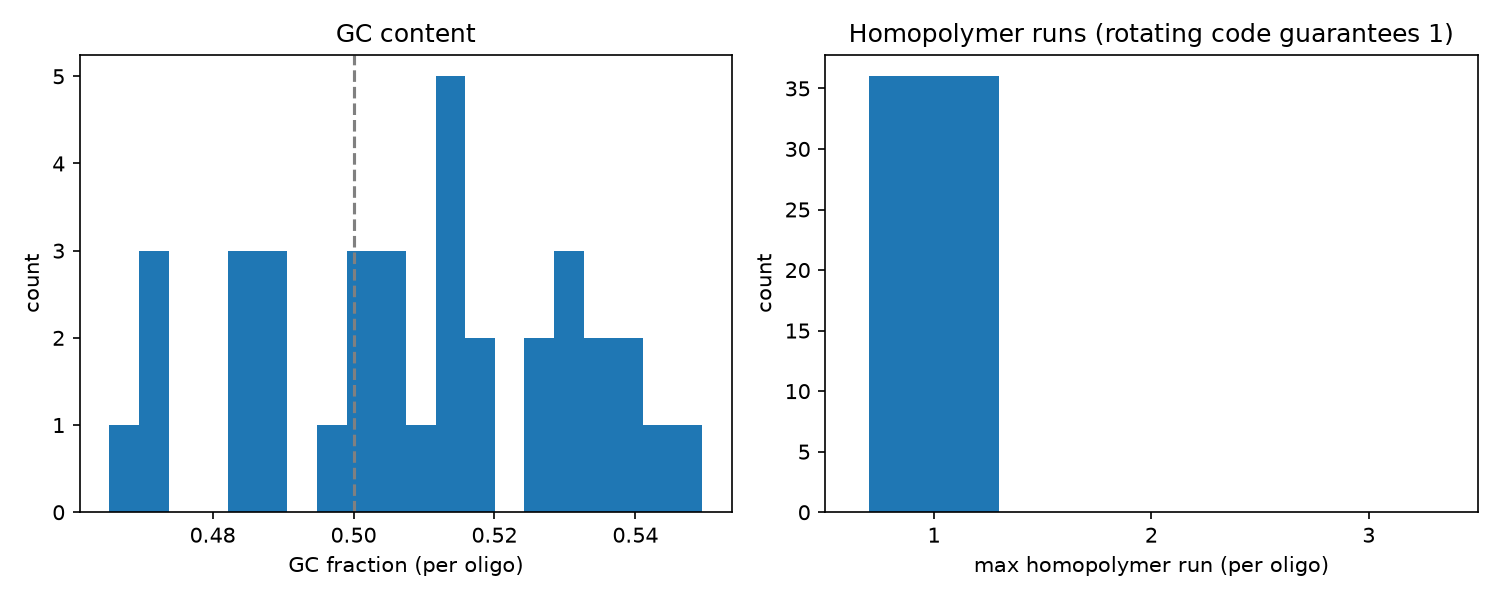
\includegraphics[width=0.9\textwidth]{constraints.png}
\caption{Per-oligo constraint satisfaction. GC content is centered near one half, and
every oligo has a maximum homopolymer run of one, the rotating codec's by-construction
guarantee. Runs are a per-oligo property and are never measured across oligo boundaries.}
\label{fig:constraints}
\end{figure}

\begin{figure}[t]
\centering
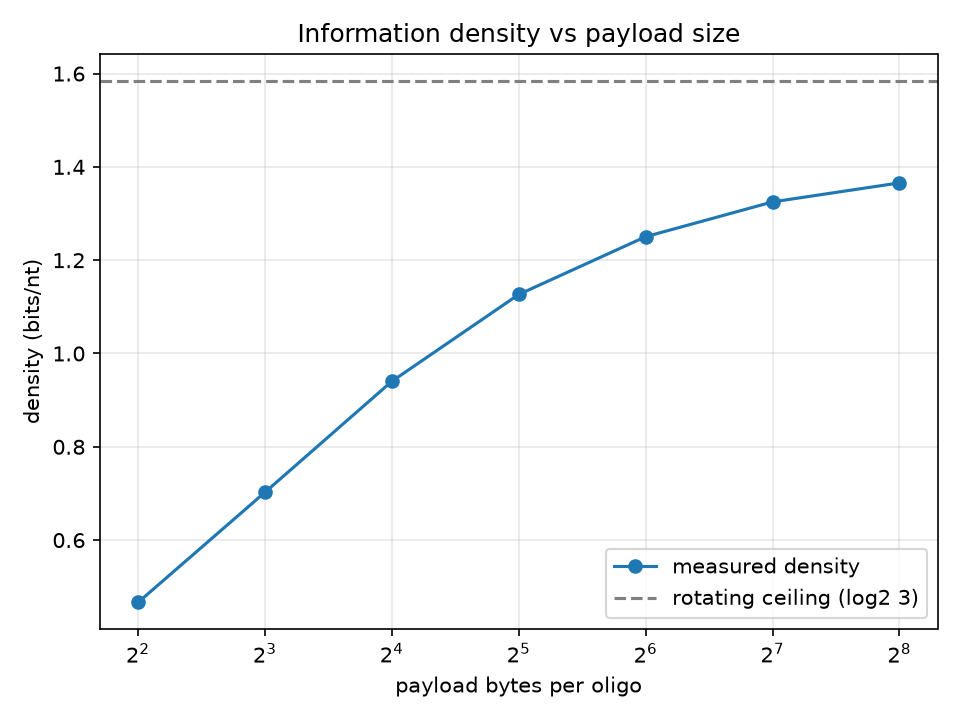
\includegraphics[width=0.7\textwidth]{density.png}
\caption{Information density versus payload size, with the data-record count held fixed so
the redundancy fraction is constant. Density rises toward the rotating ceiling
($\log_2 3 \approx \num{1.585}~bits/nt$) as the per-oligo index and CRC overhead amortize.}
\label{fig:density}
\end{figure}

\subsection{Recovery, and the role of coverage}

Recovery falls off as the per-base error rate rises, and the fall-off is governed
overwhelmingly by sequencing coverage. Figure~\ref{fig:recovery} sweeps the per-base error
rate at three coverage levels: with a single read per oligo the codec loses data almost
immediately, because a $\sim$\num{200}~nt oligo is very likely to take at least one error even
at a per-base rate of a fraction of a percent, whereas higher coverage keeps a clean read of
most oligos and extends full recovery to higher rates. This reproduces the reliance on
coverage that the wet-lab demonstrations, recovering from $\sim$\SI{1.3}{\percent} dropout in
Erlich et al. and $\sim$\SI{10}{\percent} nanopore error in Organick et al., depend on.

\begin{figure}[t]
\centering
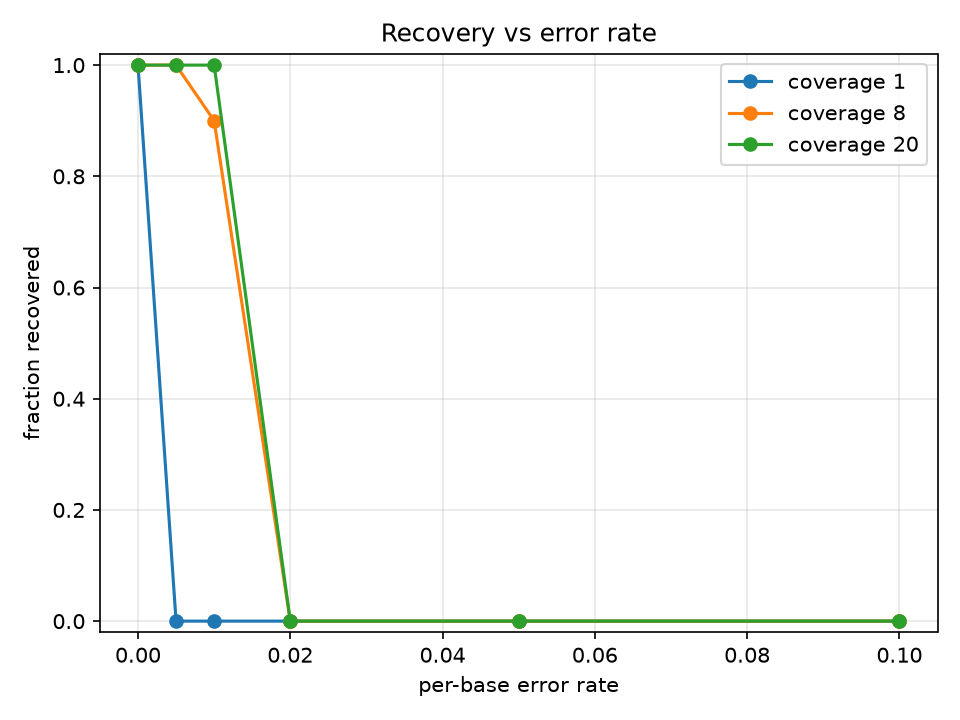
\includegraphics[width=0.7\textwidth]{recovery_vs_rate.png}
\caption{Recovery versus per-base error rate, one line per sequencing coverage. Coverage,
not coding redundancy, is the dominant recovery lever: a single read fails quickly on long
oligos, while higher coverage extends full recovery.}
\label{fig:recovery}
\end{figure}

\subsection{The density-robustness frontier}

Placing all four families on common axes, density and the highest per-base rate at which a
family fully recovers, gives the Pareto frontier of Figure~\ref{fig:pareto}. At unit
redundancy and coverage eight, the rotating families reach \num{0.634}~bits/nt and the
screening families \num{0.780}~bits/nt. Both screening families share the frontier point
(equal density, and both hold full recovery to \SI{1}{\percent} per-base error, as does
rotating-Reed-Solomon at the lower density; only rotating-fountain trails, at
\SI{0.5}{\percent}), so at this operating point the base codec and not the
error-correction family is what separates the four. The screening codec's
two-bit packing is the density lever; the base codec, not the error-correction family, moves
the point along the density axis here.

\begin{figure}[t]
\centering
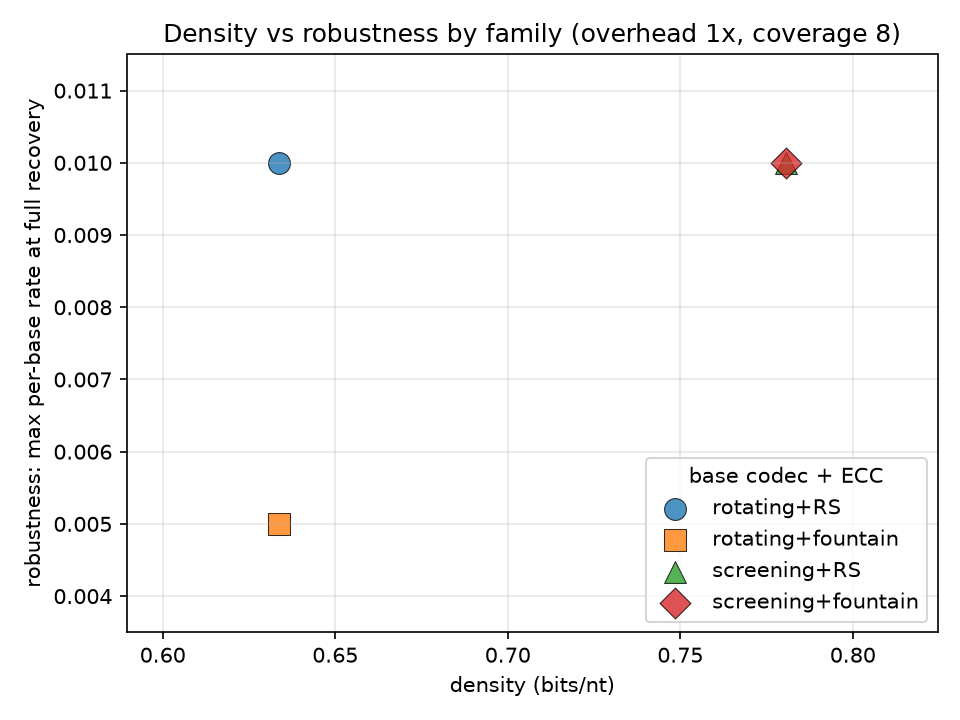
\includegraphics[width=0.7\textwidth]{pareto.png}
\caption{Density versus robustness for the four \{base codec\} $\times$ \{error-correction
family\} combinations, at matched redundancy and coverage. The screening base codec lifts
density; both screening families share the frontier point at this operating point.}
\label{fig:pareto}
\end{figure}

\subsection{Cost: coverage versus redundancy}

Sequencing coverage costs reads; coding redundancy costs synthesized bases. They are
substitutable: Figure~\ref{fig:cost} shows recovery over a grid of coverage and redundancy
at a fixed per-base rate, with the iso-recovery frontier tracing the cheapest budget that
still recovers everything. A target reliability can be met by trading reads for parity along
that frontier, and the cheapest point depends on the relative cost of sequencing and
synthesis for a given technology.

\begin{figure}[t]
\centering
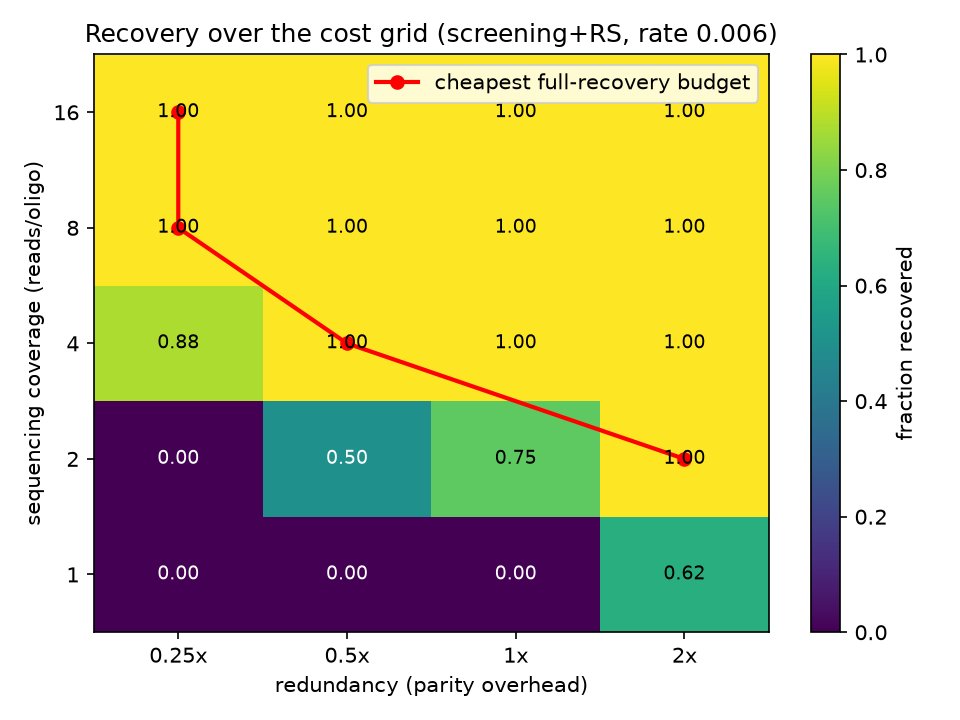
\includegraphics[width=0.75\textwidth]{cost_grid.png}
\caption{Recovery over the (coverage $\times$ redundancy) cost grid at a fixed per-base
error rate, for the screening-Reed-Solomon family. The frontier (red) is the cheapest
full-recovery budget; coverage and parity trade off against each other.}
\label{fig:cost}
\end{figure}

\subsection{Reed-Solomon versus fountain under dropout}

The two error-correction families are often presented as alternatives; the honest comparison
is less flattering to the fashionable choice. Figure~\ref{fig:dropout} sweeps redundancy at
\SI{30}{\percent} whole-oligo dropout for a large payload ($K = 188$ segments, Reed-Solomon
blocked at 64). Reed-Solomon reaches full recovery at \SI{0.75}{\times} redundancy, the
fountain code only at \SI{1.0}{\times}. Reed-Solomon is maximum-distance-separable and thus
optimal for erasures, so at fixed redundancy it matches or beats the fountain code. The
fountain code's genuine advantage is \emph{ratelessness}, the ability to emit more droplets
on demand without re-encoding when the dropout rate is unknown in advance, which a fixed-
redundancy benchmark does not reward. We report this plainly rather than imply the fountain
code dominates.

\begin{figure}[t]
\centering
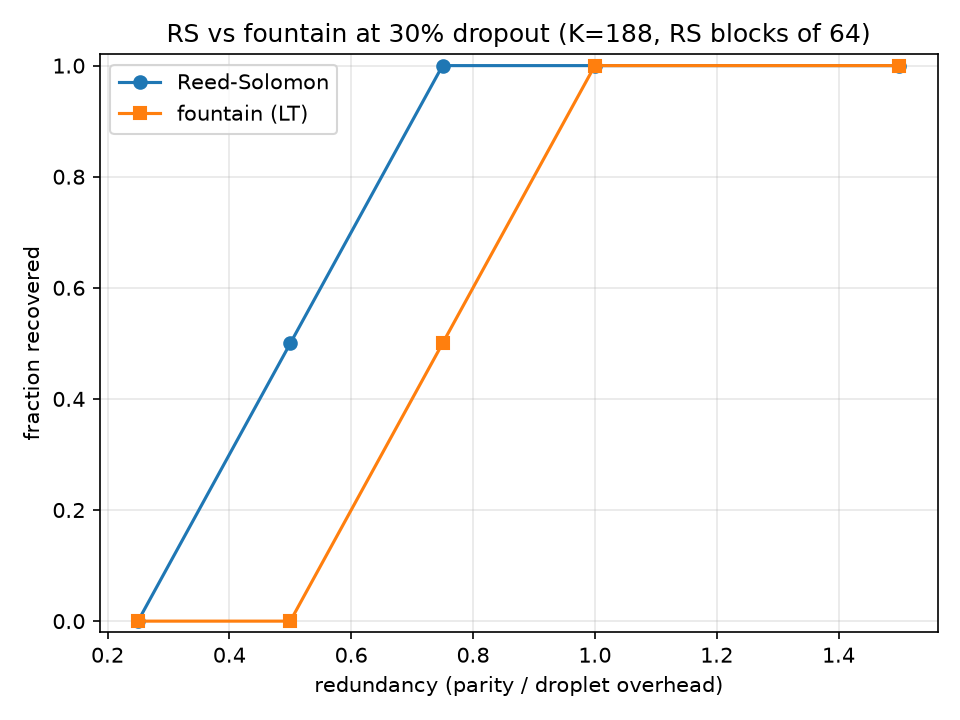
\includegraphics[width=0.7\textwidth]{dropout.png}
\caption{Reed-Solomon versus fountain recovery against redundancy at \SI{30}{\percent}
whole-oligo dropout. Reed-Solomon (MDS) reaches full recovery at lower redundancy; the
fountain code's advantage lies in ratelessness, not fixed-rate erasure efficiency.}
\label{fig:dropout}
\end{figure}

\subsection{Random access is O(1) in archive size}

Storing many equal files in one barcoded pool and retrieving a single file reads only that
file's oligos, a constant independent of how many files the pool holds, whereas decoding the
whole pool grows linearly (Figure~\ref{fig:ra}). This is the codec-level analogue of the
primer-based random access demonstrated in the wet lab~\cite{organick2018}.

\begin{figure}[t]
\centering
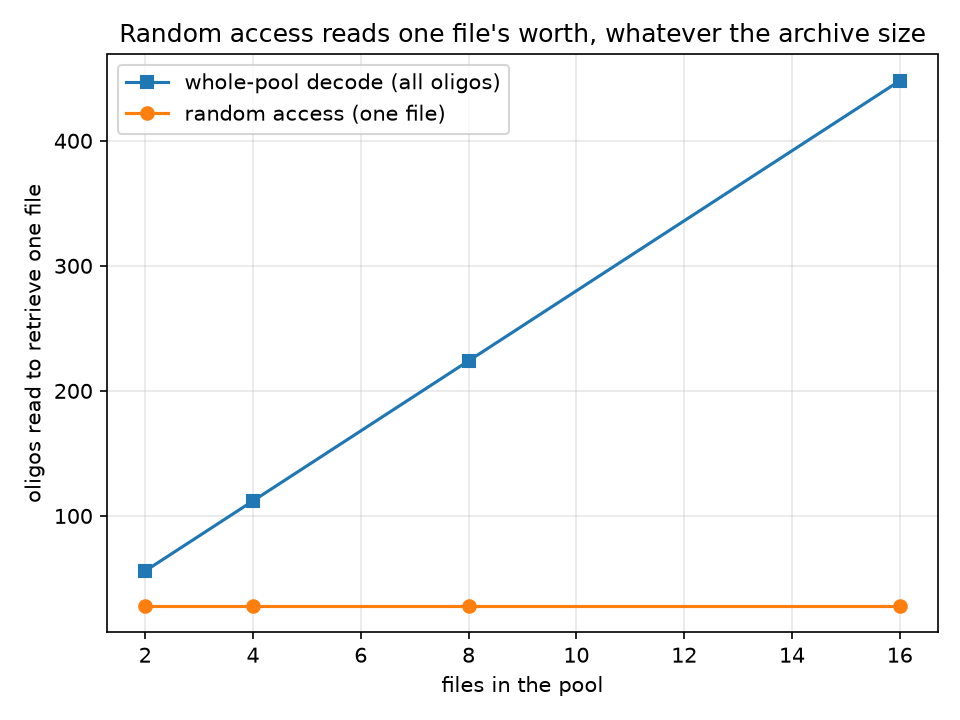
\includegraphics[width=0.7\textwidth]{random_access.png}
\caption{Per-file retrieval cost is flat in the number of files in the pool, while whole-pool
decoding grows linearly. Random access is O(1) in archive size.}
\label{fig:ra}
\end{figure}

\subsection{Indel recovery needs an error-localized base codec}
\label{sec:indel}

Figure~\ref{fig:indel} compares end-to-end deletion recovery of the detect-and-erase baseline
against the integrated marker-resync plus inner-Reed-Solomon codec, using the screening base
codec. The integrated codec holds full recovery through a per-base deletion rate of about one
percent, where detect-and-erase has already collapsed at half that rate: markers confine each
deletion to one run and the inner code corrects the residual byte errors, so the oligo
survives instead of being erased.

Crucially, this works only with an error-\emph{localized} base codec. The rotating codec
encodes each record as a single base-three integer, so one base error propagates through
base-256 carries into roughly half the record's bytes (measured 24 of 44 from a single
deletion), which no modest inner code can repair. The screening codec's two-bit-per-base
packing keeps a base error within its own byte, so the inner code succeeds. Error-localized
coding is therefore not merely a density choice but a prerequisite for in-place indel
correction, a point implicit in prior Reed-Solomon-on-blocks designs but, to our knowledge,
not measured this way. Full in-place indel correction in the Davey-MacKay watermark sense,
using soft decoding, is beyond this framework and is left as future work.

\begin{figure}[t]
\centering
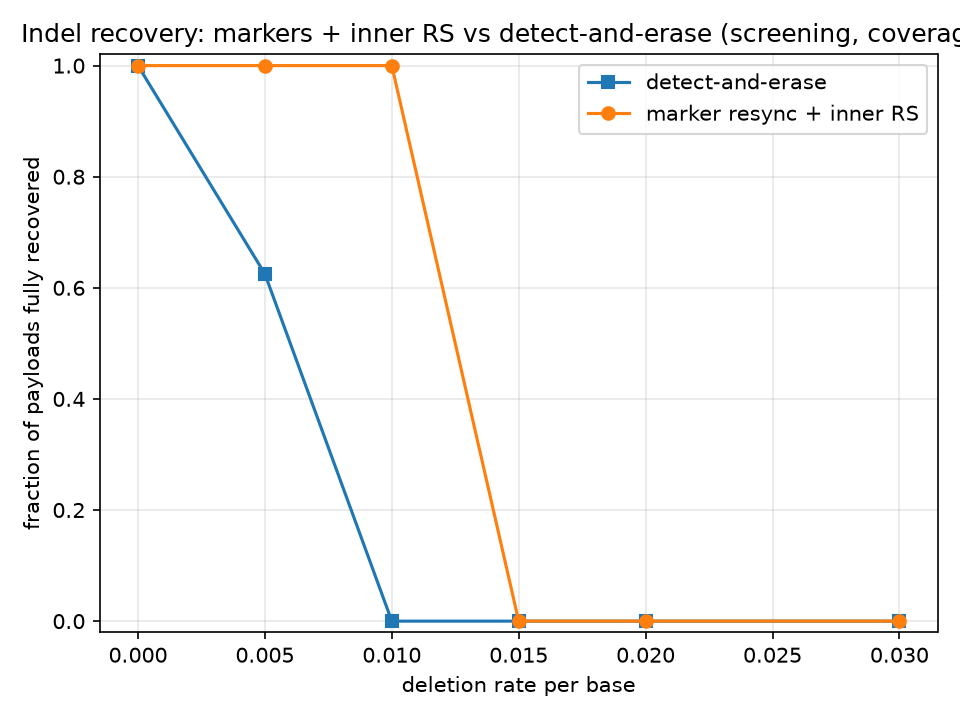
\includegraphics[width=0.7\textwidth]{indel.png}
\caption{End-to-end deletion recovery: the integrated marker-resync plus inner-Reed-Solomon
codec (screening base) recovers deletions to about one percent that the detect-and-erase
baseline loses at half that rate.}
\label{fig:indel}
\end{figure}

\subsection{Scale}

To confirm the pipeline holds beyond small synthetic payloads, we stored a real
$\sim$\num{90}~kB file, the codec's own source, in about 3000 oligos and recovered it exactly
through a realistic channel (\SI{0.2}{\percent} substitution, \SI{1}{\percent} dropout,
coverage five). The encoding achieved \num{1.22}~bits/nt at roughly four percent redundancy
with $\sim$\num{200}~nt oligos, a mean GC of \num{0.500}, and a per-oligo homopolymer run of
one.

\section{Discussion}

The comparison supports a few clear, honest conclusions. Density is set primarily by the base
codec, with the screening code's two-bit packing placing it between the Reed-Solomon and
fountain wet-lab results. Robustness is set primarily by coverage, which is substitutable with
coding redundancy along a cost frontier. Between the error-correction families, Reed-Solomon's
maximum-distance-separable property makes it match or beat the fountain code at fixed
redundancy, so the fountain code should be chosen for its ratelessness, not for a fixed-rate
efficiency it does not have. Indel correction is possible in-place, but only when the base
codec localizes errors, linking two design choices usually treated as independent. Random
access, at the codec level, costs a constant per file.

The limitations are those of a computational study. The channel is an independent-error model
with a fixed coverage, not the position-dependent, context-dependent, and over-dispersed error
process of a real sequencer; the numbers are modeled and should be read as such. The screening
codec's rejection sampling limits it to realistic oligo lengths. The marker layer is integrated
with the Reed-Solomon path but not yet with the fountain path. Full watermark-style indel
correction, an incremental experiment that would demonstrate the fountain code's ratelessness
directly, and validation against measured per-position error profiles are natural next steps.

\section{Reproducibility}

The framework is pure Python (standard library plus \texttt{numpy}, \texttt{matplotlib}, and
\texttt{reedsolo}). Every module carries assertion-based self-checks; the benchmark writes the
JSON results, the figure script regenerates every figure from those numbers, the scale
demonstration runs end to end, and a citation check verifies bibliographic integrity. The
repository is \texttt{aayushpokhrel1/dna-data-storage}; code is under the MIT License and this
text under CC-BY 4.0.

\bibliographystyle{unsrt}
\bibliography{references}

\end{document}
